\section{Durchführung}
\label{sec:Durchführung}

\subsection{Versuchsaufbau}
\label{sec:Versuchsaufbau}
%\begin{figure}
%	\centering
%	\caption{Schematische Darstellung des Versuchsaufbaus \cite{anleitung}.}
%	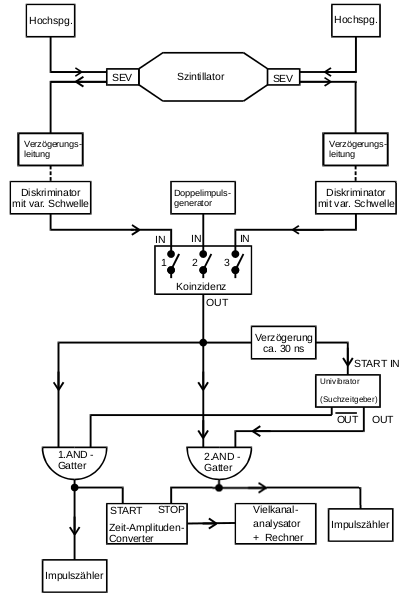
\includegraphics{Bilder/aufbau.png}
%	\label{fig:aufbau}
%\end{figure}
%
%\begin{figure}
%	\centering
%	\caption{Schematische Darstellung der Quelle zur Erzeugung radioaktiven Isotopen \cite{anleitung}.}
%	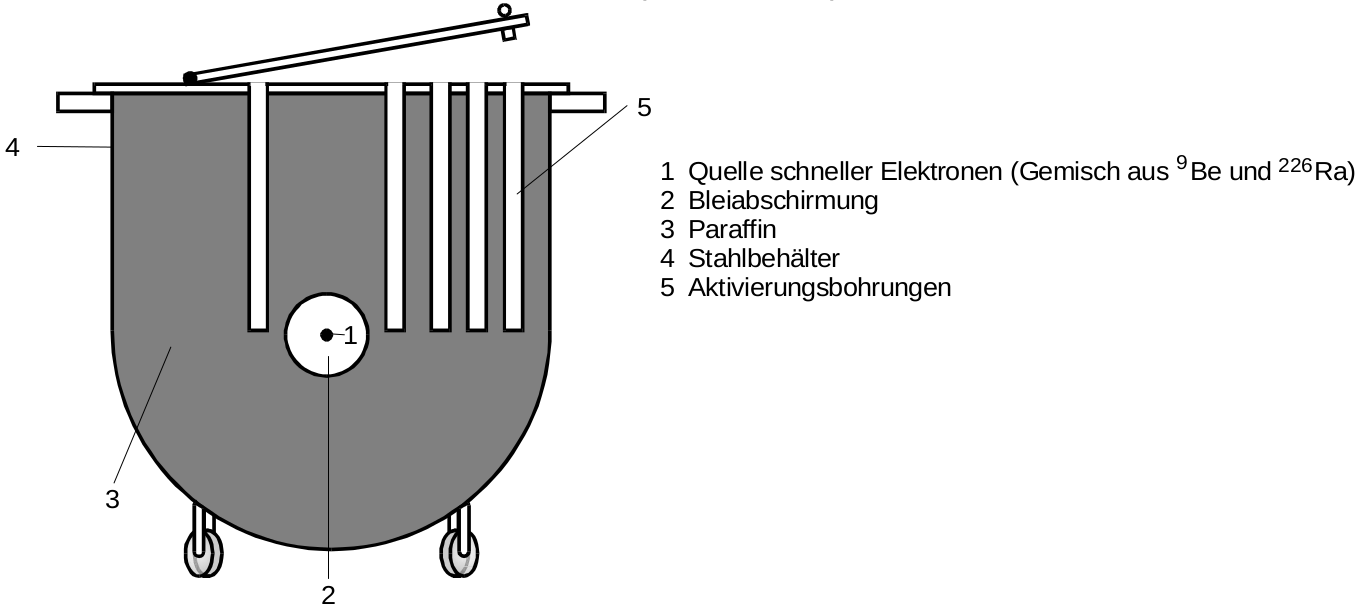
\includegraphics{content/toepfchen.png}
%	\label{fig:kochen}
%\end{figure}
%
Der Versuchsaufbau -- wie in Abbildung \ref{fig:aufbau} dargestellt -- besteht im Wesentlichen 
aus einem zerfallenden radioaktiven Isotop und einem Geiger-Müller-Zählrohr, welches die 
zerfallenden Kerne misst.
Das Geiger-Müller-Zählrohr ist entspricht einer mit Gas gefüllten Röhre. Trifft ein $\beta$-
oder $\gamma$- Teilchen auf ein Gasteilchen wird dieses ionisiert und kann aufgrund einer
anliegenden Spannung an der Röhre gemessen werden.
Dabei werden die gemessenen Zerfälle pro Messzeitintervall, welches am Zeitgeber einstellbar 
ist, an den Zählern 1 und 2 angezeigt. Nach jedem Messvorgang wird der Zähler umgeschaltet und 
der vorherige Wert auf dem aktuellen Zähler wird überschrieben. Der Versuchsaufbau ist mit
einer Blei-Abschirmung ausgestattet um die radioaktive Strahlung abzuschirmen.

Zur Erzeugung der radioaktiven Isotope wird das Objekt in Abbildung \ref{fig:kochen} verwendet.
Hierbei werden stabile Kerne mit niederenergetischen Neutronen beschossen. 
Da die Neutronen ihre Energie durch elastische Stöße an die Kerne übergeben und die maximale
Energie bei gleichen Massen der Stoßpartner erreicht wird, werden die Neutronen in einem 
Paraffinmantel gebremst, bis sie die optimale Energie besitzen.


\subsection{Versuchsbeschreibung}
\label{sec:Versuchsbeschreibung}
Mittels der Interferenz an einem optischen Gitter soll die Wellenlänge des erzeugten Laserstrahls bestimmt werden. Hierzu werden das Gitter
und ein Schirm hinter dem Laser positioniert. Aus einer Messung des Abstandes zwischen Schirm und Gitter, sowie den auftretenden Intensitätsmaxima
auf dem Schirm kann die Wellenlänge berechnet werden:
\begin{equation}
	  \lambda = \frac{g \cdot \sin(\varphi)}{n}, \quad \varphi = \arctan\left(\frac{d_n}{L} \right) ,\quad n \in \mathbb{N}
	    \label{eq:interferenz}
\end{equation}
Dabei ist $g$ die Gitterkonstante, $d_n$ der Abstand des $n$-ten Interferenzmaximums zum Hauptmaximum und $L$ der Abstand zwichen Schirm und Gitter.

Zur Untersuchung der TEM-Moden wird eine defokussierende Linse hinter den Laser gestellt, die den Laserstrahl verbreitert.
Mittels einer Mikrometerschraube kann die Photodiode
senkrecht zur Strahlachse verschoben werden und somit die Abhängigkeit zwischen Intensität und Achsenabstand untersucht werden. Zunächst
wird die Grundmode untersucht, die ohne Einsatz von Blenden gegenüber anderen Moden dominiert. Anschließeden wird die $I_{01}$-Mode
vermessen, welche eine Nullstelle bei $r = 0$ besitzt. Innerhalb des Resonators wird ein Wolframdraht so positioniert, dass die Grundmode
unterdrückt wird. Anschließend kann die $I_{01}$-Mode analog mit der Photodiode ausgemessen werden.

An den Ausgängen des Laserrohrs sind Brewster-Fenster angebracht. Hierbei handelt es sich um gläserne Platten, die
im Brewsterwinkel zu optischen Achse eingestellt werden. Gemäß den Fresnelschen Gleichungen ist der Brewsterwinkel jener Winkel, unter dem
die zur Einfallsebene parallele Komponente des elektrischen Lichtfeldes nicht reflektiert wird. Die senkrechte Komponente wird somit
durch Refelxion stark unterdrückt und das Licht linear polarisiert. Diese Gegebenheit soll
experimentell untersucht werden. Hinter den Laser wird hierzu ein drehbarer Polarisationsfilter platziert. In Abhängigkeit zum eingestellten Winkel
wird der Photostrom gemessen. Nach Malus ist die Intensität der linear polarisierten Lichtwelle hinter dem Polarisationsfilter
durch folgende Funktion zu beschreiben~\cite{malus}:
\begin{equation}
	  I(\varphi) = I_{0} \sin^2\left(\varphi + \varphi_0\right)
	    \label{eq:malus}
\end{equation}
Es sind $I_{0}$ und $\varphi_0$ die konstanten Parameter und $\varphi$ der relativ zu einer beliebigen Startachse eingestellte Winkel.

Abschließend soll die Stabilitätsbedingung \eqref{eq:stabilität} für
einen gekrümmten Spiegel $r = \SI{1.4}{\meter}$ und einen ebenen Spiegel quantitativ untersucht werden. Unter variabler Resonatorlänge $L$ wird hierzu der
Photostrom aufgezeichnet. Hierbei ist es notwendig bei jedem Abstand den Laser neu zu justieren und den Photostrom zu maximieren.
